\documentclass{article}
\usepackage{tikz}

\usetikzlibrary{quotes,arrows.meta}
\begin{document}
\begin{center}
	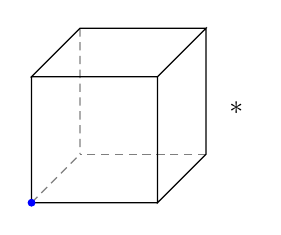
\begin{tikzpicture}[every edge quotes/.append style={auto, text=black}, scale=.4]
	\pgfmathsetmacro{\cubex}{4}
	\pgfmathsetmacro{\cubey}{4}
	\pgfmathsetmacro{\cubez}{4}
	\draw [draw=black, every edge/.append style={draw=black, densely dashed, opacity=.5}, fill=white]
	(0,0,0) coordinate (o) -- ++(-\cubex,0,0) coordinate (a) -- ++(0,-\cubey,0) coordinate (b) edge coordinate [pos=1] (g) ++(0,0,-\cubez)  -- ++(\cubex,0,0) coordinate (c) -- cycle
	(o) -- ++(0,0,-\cubez) coordinate (d) -- ++(0,-\cubey,0) coordinate (e) edge (g) -- (c) -- cycle
	(o) -- (a) -- ++(0,0,-\cubez) coordinate (f) edge (g) -- (d) -- cycle;
	\path [every edge/.append style={draw=black, |-|}];

	\draw [blue,fill] (b) circle [radius=3pt];
	\draw[] node at (2.5,-1){$\ast$};
	\end{tikzpicture}
	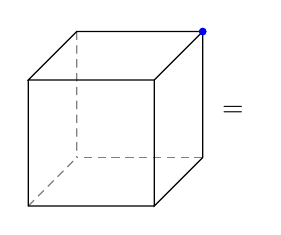
\begin{tikzpicture}[every edge quotes/.append style={auto, text=black}, scale=.4]
	\pgfmathsetmacro{\cubex}{4}
	\pgfmathsetmacro{\cubey}{4}
	\pgfmathsetmacro{\cubez}{4}
	\draw [draw=black, every edge/.append style={draw=black, densely dashed, opacity=.5}, fill=white]
	(0,0,0) coordinate (o) -- ++(-\cubex,0,0) coordinate (a) -- ++(0,-\cubey,0) coordinate (b) edge coordinate [pos=1] (g) ++(0,0,-\cubez)  -- ++(\cubex,0,0) coordinate (c) -- cycle
	(o) -- ++(0,0,-\cubez) coordinate (d) -- ++(0,-\cubey,0) coordinate (e) edge (g) -- (c) -- cycle
	(o) -- (a) -- ++(0,0,-\cubez) coordinate (f) edge (g) -- (d) -- cycle;
	\path [every edge/.append style={draw=black, |-|}];

	\draw [blue, fill] (d) circle [radius=3pt];
	\draw[] node at (2.5,-1){$=$};
	\end{tikzpicture}
	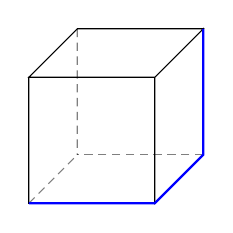
\begin{tikzpicture}[every edge quotes/.append style={auto, text=black}, scale=.4]
	\pgfmathsetmacro{\cubex}{4}
	\pgfmathsetmacro{\cubey}{4}
	\pgfmathsetmacro{\cubez}{4}
	\draw [draw=black, every edge/.append style={draw=black, densely dashed, opacity=.5}, fill=white]
	(0,0,0) coordinate (o) -- ++(-\cubex,0,0) coordinate (a) -- ++(0,-\cubey,0) coordinate (b) edge coordinate [pos=1] (g) ++(0,0,-\cubez)  -- ++(\cubex,0,0) coordinate (c) -- cycle
	(o) -- ++(0,0,-\cubez) coordinate (d) -- ++(0,-\cubey,0) coordinate (e) edge (g) -- (c) -- cycle
	(o) -- (a) -- ++(0,0,-\cubez) coordinate (f) edge (g) -- (d) -- cycle;
	\path [every edge/.append style={draw=black, |-|}];

	\draw[blue, thick] (b)--(c)--(e)--(d);
	\end{tikzpicture}
\end{center}
\end{document}